\documentclass{article}

\usepackage{amsmath}
\usepackage{amssymb}
\usepackage{graphicx}
\usepackage{fullpage}
\usepackage{parskip}
\usepackage{natbib}
\usepackage{xspace}           % Spacing in macros
\usepackage{siunitx}          % Proper formatting for units
\usepackage{float}            % For placement of table
\usepackage{caption}
\captionsetup[table]{skip=10pt}
\usepackage{booktabs}

\newcommand{\dials}{\emph{DIALS}\xspace}
\newcommand{\dxtbx}{\emph{dxtbx}\xspace}

\title{Electron diffraction data processing with \dials \\
  \large Supporting information}
\date{}

\renewcommand{\thetable}{S\arabic{table}}

%\bibliographystyle{unsrt}
%\usepackage{dcolumn,booktabs}
%\newcolumntype{d}[1]{D{.}{.}{#1}}
%\newcommand\mc[1]{\multicolumn{1}{c}{#1}} % handy shortcut macro

\begin{document}

\maketitle

\section{Simulation for comparison of ED versus MX geometry refinement}

To generate simulated spot centroid positions, we started with the real electron
diffraction example \emph{dataset 1}, consisting of a continuous rotation scan over 503 images with
an angular width of $0.076^\circ$ per image, for a total scan range of
$38.2^\circ$. We took the model for the indexed experiments and ``regularised''
the geometry of the beam and detector for the purposes of simulation, without
changing the crystal model, which had an orthorhombic unit cell with dimensions
$a=\SI{31.97}{\angstrom}$, $b=\SI{69.41}{\angstrom}$ and
$c=\SI{104.62}{\angstrom}$. To regularise the beam and detector models, we
forced the beam direction to be exactly aligned to the $-Z$ direction and
reoriented the detector model such that the beam intersected the detector in
the centre of its square window, and the detector plane was orthogonal to the
beam vector. The detector distance remained at the value of
$\SI{1890}{\milli\metre}$, as previously determined and stored in the CBF headers
for the images. The real detector consists of $2\times2$ Timepix quads with
large gaps between the active regions. For simplicity we replaced this model
with a single panel covering the total extent of the real detector, with
no parallax correction, effectively assuming it consists of a perfectly
sensitive plane of zero thickness. The updated electron diffraction geometry
was written to a new \dxtbx experiment list and then altered a second time to
produce regularised geometry for an X-ray experiment. This involved changing
the wavelength from $\SI{0.02508}{\angstrom}$ to $\SI{1.0332}{\angstrom}$ and the
detector model such that the total extent and pixel size was equivalent to a
Pilatus 6M detector at a distance of $\SI{200}{\milli\metre}$ from the sample.
This model was also written to a \dxtbx experiment list.

The regularised models were used alongside the indexed spot list from the
real data set to simulate observed centroid positions for both versions of the
experimental geometry. By using the spot list from a real experiment we ensured
a realistic distribution of strong spots versus resolution. To make sure
that the differences in refinement runs are caused only by the
diffraction geometry and not obscured by different sets of input spots, we
selected 1571 reflections that could be predicted by both versions of the
diffraction geometry.

Simulated centroid positions were calculated for each version of the geometry
by predicting their positions then adding random error. The random errors were
drawn from a normal distribution with a standard deviation of 0.25 pixels for
the $X$ and $Y$ positions and 0.25 images for the $Z$ position. For real data,
the centroid position errors in $X$, $Y$ and $Z$ are neither independent, nor
normally-distributed. However, the purpose of adding displacements to the
centroid positions was merely to ensure that refinement would proceed to
convergence with realistic final RMSDs. The centroid positions from
spot-finding result from a centre-of-gravity calculation, which also provides
estimated errors in these positions that are used to set weights in
refinement. These errors have a dependence on the found spot intensity. Rather
than simulating new error estimates, we kept the original error
estimates from spot-finding on the real data set to give a realistic
distribution of weights. The centroid $X$, $Y$ positions and their errors were
rescaled to units of millimetres for use in refinement using the pixel sizes
of $\SI{55}{\micro\metre}$ for the electron diffraction detector and
$\SI{172}{\micro\metre}$ for the X--ray detector.

\begin{figure}
  \label{fig:corrgrams-all}
  \centering
  \caption{
    Corrgrams produced for the final step of geometry refinement for simulated
    data assuming either typical electron diffraction geometry (left column)
    or X--ray diffraction geometry (right column). The top row shows
    correlation between effects of different parameters on the positional
    residuals $(X - X_o)$, the middle row shows those for the
    $(Y - Y_o)$ residuals and the lower row contains the corrgrams for the
    angular residuals $(\phi - \phi_o)$.
  }
  \includegraphics[width=0.9\textwidth]{Figures/simulation/corrgrams_all.png}
\end{figure}

\section{Processing statistics for individual datasets}

Datasets were processed individually in order to determine suitable resolution
cutoffs. These limits were then applied to unscaled data, forming the input to
the multiple dataset scaling and merging reported in the main text.

\sisetup{range-phrase=--,
         input-symbols={()}}
\begin{table}[H]
\label{tab:quality-stats-individual}
\caption{
  Data processing statistics as reported by AIMLESS for 7 individual datasets.
  Values in parentheses refer to the highest resolution shell.
}
\begin{tabular}{rSSSSSSS}
  \toprule
  Dataset & 1 & 2 & 3 & 4 & 5 & 6 & 7\\
  \midrule
  Space group & ${P 2_1 2_1 2}$ & ${P 2_1 2_1 2}$ & ${P 2_1 2_1 2}$ & ${P 2_1 2_1 2}$ & ${P 2_1 2_1 2}$ & ${P 2_1 2_1 2}$ & ${P 2_1 2_1 2}$ \\
  \addlinespace
  Unit cell\\
  $a$ ($\SI{}{\angstrom}$) & 105.12 & 104.93 & 104.25 & 105.22 & 103.47 & 105.00 & 104.14 \\
  $b$ ($\SI{}{\angstrom}$) & 68.34  & 68.51  & 67.17  & 69.65  & 64.73  & 66.50  & 68.83  \\
  $c$ ($\SI{}{\angstrom}$) & 31.98  & 32.15  & 31.55  & 32.35  & 31.84  & 31.71  & 31.73  \\
  \addlinespace
  Resolution ($\SI{}{\angstrom}$) & {31.18--2.00}  & {32.15--2.89}  & {41.18--2.85}  & {24.61--2.77}  & {27.12--2.64}  & {28.09--3.20}  & {34.71--3.00} \\
                                  & {(2.05--2.00)} & {(3.07--2.89)} & {(3.12--2.85)} & {(2.96--2.77)} & {(2.80--2.64)} & {(3.58--3.20)} & {(3.29--3.00)} \\
  \addlinespace
  $R_\textrm{merge}$ & 0.312  & 0.218   & 0.318   & 0.244   & 0.248   & 0.437   & 0.210 \\
                     &(0.538) & (0.567) & (0.538) & (0.513) & (0.465) & (0.613) & (0.504) \\
  \addlinespace
  $R_\textrm{meas}$  & 0.398  & 0.283   & 0.437   & 0.323   & 0.333   & 0.583   & 0.275  \\
                     &(0.667) & (0.692) & (0.731) & (0.659) & (0.608) & (0.816) & (0.665) \\
  \addlinespace
  $R_\textrm{pim}$   & 0.244  & 0.176   & 0.298   & 0.210   & 0.221   & 0.383   & 0.175  \\
                    & (0.389) & (0.381) & (0.492) & (0.408) & (0.387) & (0.532) & (0.430) \\
  \addlinespace
  Observations      & {18907}   & {4983}  & {2034}  & {2792}  & {3141}  & {914}   & {2012}  \\
                    & {(1512)}  & {(946)} & {(571)} & {(653)} & {(601)} & {(276)} & {(513)} \\
  \addlinespace
  Completeness (\%) & 50.1    & 42.0   & 26.4   & 26.6   & 29.7   & 17.3   & 25.9 \\
                    & (48.4)  & (41.7) & (28.6) & (28.7) & (30.2) & (18.1) & (28.1) \\
  \addlinespace
  Multiplicity      &  2.4     & 2.2   & 1.5    & 1.7    & 1.6    & 1.4   &  1.6  \\
                    & (2.8)   & (2.7) & (1.6)   & (2.0)  & (1.9)  & (1.5) & (1.6) \\
  \addlinespace
  $\langle I/\sigma(I) \rangle$ & 2.0   & 2.7   & 2.0   & 2.2   & 1.8   &  2.1  & 2.2 \\
                                & (1.4) & (1.5) & (1.1) & (1.5) & (1.4) & (1.0) & (1.0) \\
  \addlinespace
  $CC_{{1}/{2}}$ (\%) & 89.3  & 91.6   & 65.5   & 88.8   & 85.6   & 73.1   & 92.9 \\
                      &(53.1) & (52.8) & (51.3) & (58.8) & (59.2) & (55.4) & (46.4) \\
  \bottomrule
\end{tabular}

\end{table}

%\bibliography{dials}

\end{document}
